\documentclass[ignorenonframetext,10pt,aspectratio=169]{beamer}

\usepackage{umut}
\usepackage{umuttr}
\usepackage[utf8]{inputenc}
\usepackage{uling}
\usepackage{uprog,usynsem}
\usepackage{fancyvrb}
\usepackage{natbib,unatbib}
\usepackage{linguex}
         \renewcommand{\refdash}{}
\usepackage{ubeamer}
\usepackage{verbatim}
\usepackage{graphicx}

\usepackage{tikz-qtree}
\usetikzlibrary{er,positioning}

\title{Applicative programming: basic tools}
\author{\  \\ \vspace{20pt} Umut \"Ozge\\  }

\date{COGS 502: Symbols and Programming \\ METU, Informatics}

\begin{document}

\begin{frame}\frametitle{}
\thispagestyle{empty}
\maketitle
\end{frame}

\begin{frame}[t,plain]{Global variables}
\vspace{10pt}
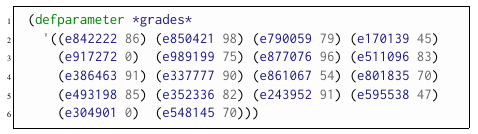
\includegraphics[scale=0.7]{img/defpar.png}

\end{frame}

\begin{frame}[t,plain]{MAPCAR}


\end{frame}

\begin{frame}[t,plain]{LAMBDA}

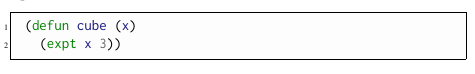
\includegraphics[scale=0.7]{img/defcube.png}
\pause
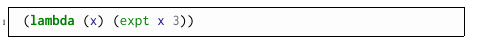
\includegraphics[scale=0.7]{img/lamcube.png}
\pause
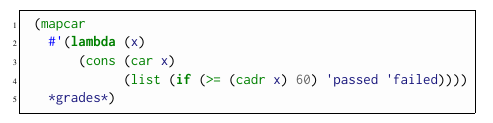
\includegraphics[scale=0.7]{img/maplam.png}
\end{frame}


\begin{frame}[t,plain]{REDUCE}

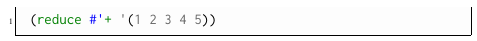
\includegraphics[scale=0.7]{img/redplus.png}
\pause
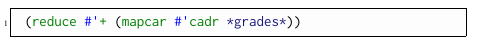
\includegraphics[scale=0.7]{img/redgrades.png}
\pause
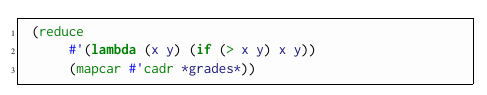
\includegraphics[scale=0.7]{img/redmax.png}

\end{frame}

\begin{frame}[t,plain]{REMOVE-IF}

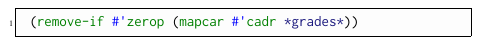
\includegraphics[scale=0.7]{img/remif1.png}
% \pause
% 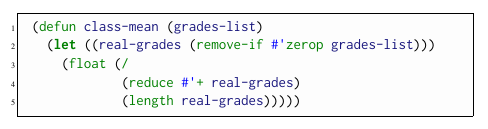
\includegraphics[scale=0.7]{img/remif2.png}

\end{frame}

\begin{frame}[t,plain]{MAKE-LIST}


\end{frame}

\end{document}
